%!TEX root = mainfile.tex

\section{Gravitational Lensing} % (fold)
\label{sec:gravitational_lensing}

    \subsection{Introduction} % (fold)
    \label{sub:introduction}
        Contrary to a popularly held belief that Newton refers to gravitational lensing in his publication ``Opticks''\cite{Newton_Opticks} (put into context, it is clear that he was discussing diffraction), the first person to allude directly to the bending of light due to gravitational attraction was Henry Cavendish. Around the turn of the 19th century Cavendish used Newton's corpuscular theory to correctly calculate the bending of light around a massive object.  Around the same time, German astronomer Johann Soldner was independently addressing the same problem\cite{Soldner} and although his results were similar to those obtained by Cavendish, his method was fundamentally flawed due to incorrect assumptions\cite{Conceptual_origins_of_GL}.

        The subject of gravitational lensing was then largely put to rest until 1915 when Einstein postulated his theory of general relativity, from which it is clear that massive objects will cause light to bend as a result of the curvature of spacetime. Despite having complete and correct calculations of the phenomenon of gravitational lensing, including the lens equation and the position of images, Einstein displayed very little interest in it. He mentions it only briefly in his notebooks and published a single, very short discussion in science magazine upon the request of a friend at the end of which he dismissively comments that there is “no great chance of this phenomenon being observed”\cite{Einstein_science_magazine}.

        During a solar eclipse in 1919, Eddington measured the positions of stars lying close to the sun and observed that their positions appeared at a greater distance from the sun than expected, thereby giving the first experimental evidence for the bending of light around the sun\cite{Eddington_GL_evidence}. 5 years later, Chwolson published a paper on the idea that `fake double stars' may be observed as a result of the gravitational lensing effect and postulated that if source, lens and observer are perfectly aligned then a `Chwolson ring', later renamed `Einstein ring', would form around the lens\cite{Conceptual_origins_of_GL}.

        The true pioneer of the subject, however, is generally considered to be Czech astronomer\cite{F_Link_GL} Frantisek Link. Through detailed calculations of image magnification and positions, Link concluded that in some cases gravitational lensing would make faint sources visible. Optimistic about the possibility of observing these sources, particularly for spiral nebulae, he published a detailed paper on his wide ranging calculations which included the deflection undergone by light rays passing massive objects, the resulting change in intensity of sources and the invariance of source surface brightness. Following this, there was again a period of lack of interest, during which only a few papers were published on the subject until the discovery of the first lens in 1979 by Walsh, Carswell and Weymann. From here onwards, it became a topic of intense interest to astronomers and many more lenses and faint sources have since been discovered\cite{Conceptual_origins_of_GL}.
    % subsection introduction (end)

    \subsection{Concept} % (fold)
    \label{sub:concept}
        The bending of light around a massive object is a direct result of Einstein's theory of relativity and the curvature of spacetime. This effect can cause massive objects to act as lenses for background sources by bending the light such that rays that otherwise would not have been detected converge at the observer, resulting in a brighter image being observed. The increase in flux reaching the observer can result in significant magnification of a source, for example, one of the most distant objects known was observed behind the cluster Abell 2218 with a magnification factor of 30, equivalent to a decrease of 3.7 AB magnitudes\cite{Distant_object_Abell2218}. Studying the magnification and properties of the images can yield information about both the lens and the source, making it an extremely useful tool\cite{Hartle}.
        \begin{figure}[ht]
            \centering
                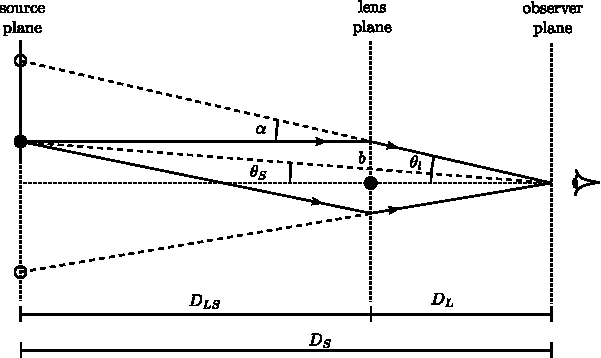
\includegraphics[width=0.6\textwidth]{../Images/Lensing_light_bending.pdf}
            \caption[Diagram of a gravitational lens]{In this schematic diagram of a gravitational lens, DL, DS and DLS represent the observer-lens, observer-source and lens-source distances respectively. $\theta_i$ is the image angle and $\theta_S$ the source angle, relative to the observer-lens axis. The light ray (solid line) passes by the lens at impact parameter $b$ and as a result is deflected by angle $\alpha$, converging with a second ray at the observer. The dotted lines indicate the position at which the images are observed\cite{Lensing_light_bending_diagram}.\label{fig:Lensing_light_bending}}
        \end{figure}
        Lensing in which multiple images are formed and the source is significantly magnified is known as strong lensing. For this to occur, the lens must have a high mass and the source angle $\theta_S$ must be small. The schematic diagram in figure~\ref{fig:Lensing_light_bending} shows a gravitational lens acting on light from a background source in such a way as to form two images. The distances between observer, lens and source are so large in comparison to the impact parameter $b$ that to good approximation, the lens radius is negligible and it can be modelled as a thin lens. It is therefore reasonable to assume that the light travels in straight lines at all times except in the lens plane where the complete deflection occurs. Furthermore, it can be assumed that for all values of $b$, the deflection angle is given by
        \begin{align}
            \alpha &= \frac{4GM}{c^2 b}
        \end{align}
        where $M$ is the mass of the lens, c the speed of light and $G$ is the gravitational constant. In realistic lensing situations, all the angles shown in figure~\ref{fig:Lensing_light_bending} are very small, hence the small angle approximation can be applied to yield the lens equation
        \begin{align}
            \theta_i D_S &= \theta_S D_S + \alpha D_{LS}
        \end{align}
        and also to approximate the impact parameter to $b\approx\theta_i DL$, it follows that
        \begin{align}
            \theta_i &= \theta_S + \frac{\theta_E^2}{\theta_i} \label{eq:einstein_angle}
        \end{align}
        where $\theta_E$ corresponds to the Einstein angle (or Einstein radius), given by
        \begin{align}
            \theta_E &= \frac{4GM}{c^2}\frac{D_{LS}}{D_L D_S}
        \end{align}
        sets the characteristic angular scale for any lensing system\cite{Hartle}.

        In the rare case that the source, lens and observer in a lensing system are perfectly aligned, a ring of light is observed around the lens, known as an Einstein ring. This ring will be at a constant distance from the centre of the ring equal to the Einstein radius. More commonly, the source is offset from the observer lens axis, resulting in the formation of multiple images. The number of images formed by a lens is always odd, however, using the limit of a small but finite spherical lens, one image is formed directly behind the lens and is not observed since the lens will always be brighter.
        \begin{figure}[ht]
            \centering
                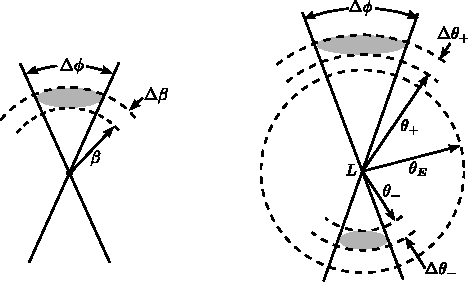
\includegraphics[width=0.6\textwidth]{../Images/Lensing_image_positions2.pdf}
                \caption[Schematic diagram of location of images]{Schematic diagram of location of images. The centre labelled L represents the observer-lens axis. The diagram on the left shows what would be observed if the lens was not present. The right hand diagram includes the effects of lensing\cite{Hartle}.\label{fig:Lensing_image_positions2}}
        \end{figure}

        In the case shown in Figure lensing image positions where two visible images are observed, one image will form inside the Einstein radius ($\theta_{i+}$) and the other outside ($\theta_{i+}$). The positions of these two images are calculated by solving the equation~\ref{eq:einstein_angle} giving
        \begin{align}
            \theta_{i\pm} &= \frac{1}{2}\left( \theta_S \pm {(\theta_S^2 + 4\theta_E^2)} ^{\frac{1}{2}} \right) \label{eq:image_position}
        \end{align}
        yielding the positions of the two images as shown in figure lensing image positions– one inside the Einstein radius, the other outside. Unlike optical lenses, gravitational lenses are achromatic, so the frequency of the light has no effect on the position of the images. As a result, images of the same object have exactly the same spectra and can easily be identified\cite{Hartle}.

        The azimuthal angle $\phi$ remains unchanged with and without the lens but as shown in figure lensing image positions, the polar angle and the width of the images are changed. The observed images are, therefore, stretched out into arcs and at any given radius will have the same curvature of a circle with origin at the centre of the lens\cite{Image_arc_curvature}. The change in the polar angle $\theta$ can be calculated by differentiating equation~\ref{eq:image_position}, giving
        \begin{align}
            \Delta\theta_{i\pm} &= \frac{1}{2}\left( 1 \pm \frac{\theta_S}{(\theta_S^2 +4\theta_E^2)}^{\frac{1}{2}} \right) \Delta\theta_S
        \end{align}

        This shape distortion results from the fact that the sources are not point objects but in fact have light coming from a large area of the sky. The light from each end of the object will take different paths through the sky and will pass the lens at a different distance. The light will therefore be bent differently for different parts of the galaxy and the shape is distorted\cite{Arc_shapes_site}.

        The magnification of the source is given by the ratio of the image brightness to the source brightness. The surface brightness of any given source remains constant\cite{Hartle} but the effective solid angle $\Omega$ subtended by the detector is increased by the lens, hence the flux received by the detector, given by
        \begin{align}
            F &= (\text{surface brightness}) \times \Omega
        \end{align}
        is also increased. Since the observed brightness of the source depends on the flux, the magnification is given by
        \begin{align}
            \mu &= \frac{F_{i\pm}}{F_S} = \frac{\Omega_{i\pm}}{\Omega_S}
        \end{align}
        Since in the small angle approximation, $\sin\theta \approx \theta$, the solid angles for the image and source are given by $\theta_{i\pm}\Delta\theta_{i\pm}\Delta\phi$ and $\theta_S \Delta_S \phi$ respectively. Given that $\Delta\phi$ is the same for both images, the magnification can be expressed as
        \begin{align}
            \mu_{\pm} &= \left| \left( \frac{\theta_{i\pm}}{\theta_S} \dx{\theta_{i\pm}}{\theta_S} \right) \right| \\
            &=\frac{1}{4}\left( \frac{\theta_S}{{(\theta_S^2 +4\theta_E^2)}^{\frac{1}{2}}} + \frac{{(\theta_S^2 +4\theta_E^2)}^{\frac{1}{2}}}{\theta_S} \pm 2 \right)
        \end{align}
        The change in AB magnitude is then found using equation~\ref{eq:magnitude_conversion}\cite{IOP_ABmagnification_site},
        \begin{align}
            \Delta m &= -2.5\log(\mu) \label{eq:magnitude_conversion}
        \end{align}
        The smaller the angle between the observer-lens axis and the source $\theta_S$, the greater the magnification of the source.
    % subsection concept (end)

% section gravitational_lensing (end)
